\section{Ausführen}\label{ProjektStart}
Im folgenden Abschnitt wird kurz erklärt, wie man zunächst den Server startet und anschließen die Ionic-Anwendung über einen Browser darstellen kann. Sollte VS Code als Entwicklungsumgebung genutzt werden, bietet es sich an eine Instanz von VS Code für das Backend und eine Instanz von VS Code für das Frontend zu starten.

\subsection{Start Backend}
\begin{enumerate}
    \item VS Code bietet im Reiter den Punkt "Terminal"{} an. Darüber kann direkt in VS Code ein Terminal geöffnet werden. Das Terminal befindet sich schon im richtigen Ordner. Alternativ kann auch die Eingabeaufforderung oder die PowerShell gestartet werden und in den Projektordner "Backend" navigiert werden.
    
    \item Im ersten Schritt wechseln Sie in den Ordner vorhanden "rest\_controller"{}.\\Befehl: "cd rest\_controller"{}
    
    \item Zunächst muss das Projekt kompiliert werden. Dies kann per Befehl "mvn clean | mvn package"{} ausgeführt werden.\\\textcolor{red}{Wichtig:} Maven muss auf dem System vorhanden und über die Umgebungsvariablen dem System bekannt sein.
    
    \item Wurde das Projekt erfolgreich kompiliert, kann der Server per folgendem Befehl gestartet werden: "docker-compose up --build"{}\\
    Auch hier sei zu beachten, das sich zum einen das Terminal im Ordner "rest\_controller"{} befinden sollte und zum anderen der Docker-Deamon (Docker.exe) gestartet ist. Das Starten des Servers kann je nach Hardware einige Minuten benötigen.
\end{enumerate}


\subsection{Start Frontend}

\begin{enumerate}
    \item Auch beim Starten des Frontends wird zunächst ein neues Terminal geöffnet. Wahlweise durch VS Code oder durch Starten eines eigenen Terminal Clients. 
    
    \item Zum starten der Ionic-Anwendung muss jedoch nur der Befehlt "{}ionic serve --lab"{} ausgeführt werden. Ionic übernimmt alle weiteren Schritte zum Starten der Ionic-Anwendung. Diese wird auch automatisch im Webbrowser geöffnet, sobald alle Daten kompiliert wurden. Wird der Befehlt "{}ionic serve --lab"{} zum ersten Mal ausgeführt, kann es sein, dass Sie noch einige Abhängigkeiten installieren müssen.
    
\end{enumerate}

\subsection{Fehlerbehandlung}\label{SpringFehler}
Ein möglicher Fehler der Auftreten kann, wäre dass Spring Boot den Pfad zur JDK nicht findet und beim compilieren der Spring Boot Anwendung mit der Fehlermeldung "No compiler is provided in this environment. Perhaps you are running on a JRE rather than a JDK?"{} abstürzt. 
\\\\
In diesem Fall muss in der pom-Datein des Servers die Pfad-Angabe des JDK angepasst werden. Die pom-Datei befindet sich im Ordner "Backend\textbackslash{}rest\_controller\textbackslash{}"{}.

\begin{center}
    \begin{minipage}[t]{0.8\textwidth}
        \centering
        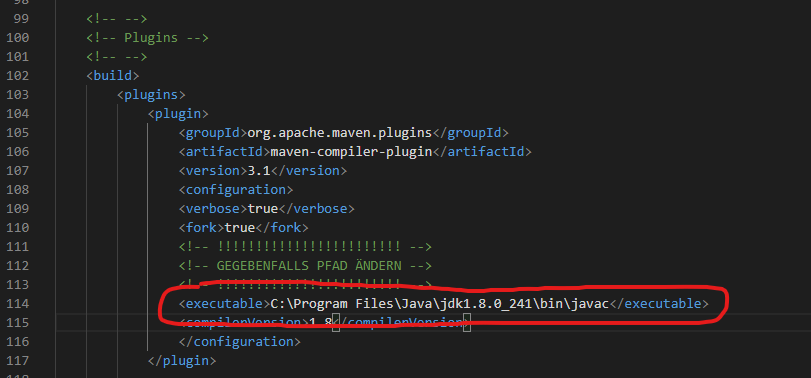
\includegraphics[width=(\textwidth)]{Kapitel3/SpringFehler.png}
        \captionof{figure}{Path-Angabe zur JDK muss angepasst werden.}
        \label{ContainerConfig}
    \end{minipage}
\end{center}
Ein weiterer Fehler könnte der sogenannte CORS-Fehler der Ionic beim Ausführen der Ionic-Anwendung im Browser auftreten kann. Die gemeinsame Nutzung von Ressourcen aus verschiedenen Quellen (Cross-Origin Resource Sharing, CORS) ist ein Standard, der es einem Server erlaubt, die Politik der gleichen Herkunft zu lockern. Dies wird verwendet, um einige Anfragen aus verschiedenen Quellen explizit zuzulassen und andere abzulehnen. Wenn eine Website beispielsweise einen integrierbaren Dienst anbietet, kann es notwendig sein, bestimmte Einschränkungen zu freizugeben. \cite{Mozilla.10.04.2020}\\\\Eine mögliche Fehler-Quelle kann sein, dass der Browser CORS-Anfrage ablehnt. Je nach Browser zum Beispiel Chrome werden einige Plugins angeboten, welche ermöglichen CORS-Anfrage zu versenden und zu empfangen. Für Google Chrome wäre dies "Allow CORS: Access-Control-Allow-Origin"{}. Aber auch für Firefox sollte ein ähnliches Plugin zur Verfügung stehen.